\documentclass{article}
\usepackage[paperwidth=7.2in,paperheight=3.1in,margin=0.08in]{geometry}
\usepackage{tikz}
\usepackage{xcolor}
\usepackage{times}
\pagestyle{empty}

\definecolor{blue300}{HTML}{9FD2F5}
\definecolor{cardblue}{HTML}{2D5F9A}
\definecolor{attrgreen}{HTML}{2F855A}
\definecolor{edgegray}{HTML}{5A6470}
\definecolor{softgray}{HTML}{F3F5F7}

\usetikzlibrary{arrows.meta,positioning,shapes.geometric}

\tikzset{
  cardnode/.style={
    rectangle, rounded corners=5pt, draw=cardblue, very thick,
    fill=blue300!45, align=center, text width=1.35in,
    minimum height=0.52in, font=\bfseries\small
  },
  attrnode/.style={
    rectangle, rounded corners=4pt, draw=attrgreen, thick,
    fill=attrgreen!10, align=center, text width=1.12in,
    minimum height=0.34in, font=\scriptsize
  },
  edgelabel/.style={font=\tiny, fill=white, inner sep=1pt, text=edgegray},
  arrow/.style={-Latex, thick, draw=edgegray},
  panel/.style={
    rectangle, rounded corners=5pt, draw=black!25, fill=softgray,
    inner sep=6pt
  }
}

\begin{document}
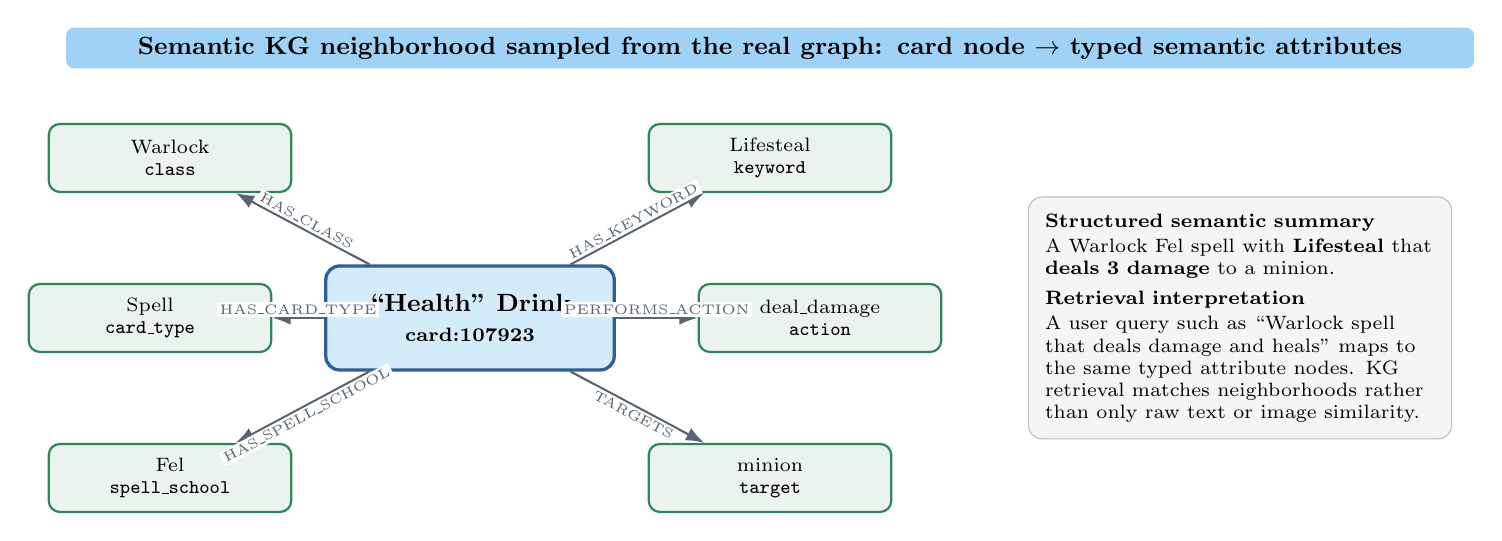
\begin{tikzpicture}[x=1in,y=1in]
  \node[fill=blue300, rounded corners=3pt, text width=6.95in, align=center, font=\bfseries\small] at (3.55,2.9)
    {Semantic KG neighborhood sampled from the real graph: card node $\rightarrow$ typed semantic attributes};

  \node[cardnode] (card) at (2.05,1.55) {``Health'' Drink\\ \scriptsize card:107923};

  \node[attrnode] (warlock) at (0.55,2.35) {Warlock\\ \texttt{class}};
  \node[attrnode] (spell) at (0.45,1.55) {Spell\\ \texttt{card\_type}};
  \node[attrnode] (fel) at (0.55,0.75) {Fel\\ \texttt{spell\_school}};
  \node[attrnode] (lifesteal) at (3.55,2.35) {Lifesteal\\ \texttt{keyword}};
  \node[attrnode] (damage) at (3.8,1.55) {deal\_damage\\ \texttt{action}};
  \node[attrnode] (minion) at (3.55,0.75) {minion\\ \texttt{target}};

  \draw[arrow] (card) -- node[edgelabel, above, sloped] {HAS\_CLASS} (warlock);
  \draw[arrow] (card) -- node[edgelabel, above] {HAS\_CARD\_TYPE} (spell);
  \draw[arrow] (card) -- node[edgelabel, below, sloped] {HAS\_SPELL\_SCHOOL} (fel);
  \draw[arrow] (card) -- node[edgelabel, above, sloped] {HAS\_KEYWORD} (lifesteal);
  \draw[arrow] (card) -- node[edgelabel, above] {PERFORMS\_ACTION} (damage);
  \draw[arrow] (card) -- node[edgelabel, below, sloped] {TARGETS} (minion);

  \node[panel, text width=1.95in, align=left, font=\scriptsize] at (5.9,1.55) {
    \textbf{Structured semantic summary}\\[0.15em]
    A Warlock Fel spell with \textbf{Lifesteal} that \textbf{deals 3 damage} to a minion.\\[0.35em]
    \textbf{Retrieval interpretation}\\[0.15em]
    A user query such as ``Warlock spell that deals damage and heals'' maps to the same typed attribute nodes. KG retrieval matches neighborhoods rather than only raw text or image similarity.
  };
\end{tikzpicture}
\end{document}
